
% Aberdeen style guide should be followed when using this
% layout. Their template powerpoint slide is used to extract the
% Aberdeen color and logo but is otherwise ignored (it has little or
% no formatting in it anyway).
%
% http://www.abdn.ac.uk/documents/style-guide.pdf

%%%%%%%%%%%%%%%%%%%% Document Class Settings %%%%%%%%%%%%%%%%%%%%%%%%%
% Pick if you want slides, or draft slides (no animations)
%%%%%%%%%%%%%%%%%%%%%%%%%%%%%%%%%%%%%%%%%%%%%%%%%%%%%%%%%%%%%%%%%%%%%%
%Normal document mode
\documentclass[10pt,compress]{beamer}
%Draft or handout mode
%\documentclass[10pt,compress,handout]{beamer}
%\documentclass[10pt,compress,handout,ignorenonframetext]{beamer}
\usepackage{lmodern}

\usepackage{xcolor}
\usepackage{float} 

\usepackage[]{algorithm2e} 
\usepackage{algorithmic}

\newlength{\overwritelength}
\newlength{\minimumoverwritelength}
\setlength{\minimumoverwritelength}{1cm}
\newcommand{\overwrite}[3][red]{%
  \settowidth{\overwritelength}{$#2$}%
  \ifdim\overwritelength<\minimumoverwritelength%
    \setlength{\overwritelength}{\minimumoverwritelength}\fi%
  \stackrel
    {%
      \begin{minipage}{\overwritelength}%
        \color{#1}\centering\small #3\\%
        \rule{1pt}{9pt}%
      \end{minipage}}
    {\colorbox{#1!50}{\color{black}$\displaystyle#2$}}}



%%%%%%%%%%%%%%%%%%%% General Document settings %%%%%%%%%%%%%%%%%%%%%%%
% These settings must be set for each presentation
%%%%%%%%%%%%%%%%%%%%%%%%%%%%%%%%%%%%%%%%%%%%%%%%%%%%%%%%%%%%%%%%%%%%%%
\newcommand{\shortname}{Dr Jeff Gomes}
\newcommand{\fullname}{Dr Jeff Gomes}
\institute{School of Engineering}
\newcommand{\emailaddress}{jefferson.gomes@abdn.ac.uk}
\newcommand{\logoimage}{./FigBanner/UoAHorizBanner}
\title{Advanced Chemical Engineering (EG5597)}
\subtitle{Computational Methods for Fluid Dynamics -- Introduction}
\date[25/04 - 09/05/2014]{25/04 - 09/05/2014}

%%%%%%%%%%%%%%%%%%%% Template settings %%%%%%%%%%%%%%%%%%%%%%%%%%%%%%%
% You shouldn't have to change below this line, unless you want to.
%%%%%%%%%%%%%%%%%%%%%%%%%%%%%%%%%%%%%%%%%%%%%%%%%%%%%%%%%%%%%%%%%%%%%%
\usecolortheme{whale}
\useoutertheme{infolines}

% Use the fading effect for items that are covered on the current
% slide.
\beamertemplatetransparentcovered

% We abuse the author command to place all of the slide information on
% the title page.
\author[\shortname]{%
  \fullname\\\ttfamily{\emailaddress}
}


%At the start of every section, put a slide indicating the contents of the current section.
\AtBeginSection[] {
  \begin{frame}
    \frametitle{Section Outline}
    \tableofcontents[currentsection]
  \end{frame}
}

% Allow the inclusion of movies into the Presentation! At present,
% only the Okular program is capable of playing the movies *IN* the
% presentation.
\usepackage{multimedia}
\usepackage{animate}

%%%%% Color settings
\usepackage{color}
%% The background color for code listings (i.e. example programs)
\definecolor{lbcolor}{rgb}{0.9,0.9,0.9}%
\definecolor{UoARed}{rgb}{0.64706, 0.0, 0.12941}
\definecolor{UoALight}{rgb}{0.85, 0.85, 0.85}
\definecolor{UoALighter}{rgb}{0.92, 0.92, 0.92}
\setbeamercolor{structure}{fg=UoARed} % General background and higlight color
\setbeamercolor{frametitle}{bg=black} % General color
\setbeamercolor{frametitle right}{bg=black} % General color
\setbeamercolor{block body}{bg=UoALighter} % For blocks
\setbeamercolor{structure}{bg=UoALight} % For blocks
% Rounded boxes for blocks
\setbeamertemplate{blocks}[rounded]
% Numbering captions
\setbeamertemplate{caption}[numbered]%\numberwithin{figure}{section}
%%%%% Font settings
% Aberdeen requires the use of Arial in slides. We can use the
% Helvetica font as its widely available like so
% \usepackage{helvet}
% \renewcommand{\familydefault}{\sfdefault}
% But beamer already uses a sans font, so we will stick with that.

% The size of the font used for the code listings.
\newcommand{\goodsize}{\fontsize{6}{7}\selectfont}

% Extra math packages, symbols and colors. If you're using Latex you
% must be using it for formatting the math!
\usepackage{amscd,amssymb} \usepackage{amsfonts}
\usepackage[mathscr]{eucal} \usepackage{mathrsfs}
\usepackage{latexsym} \usepackage{amsmath} \usepackage{bm}
\usepackage{amsthm} \usepackage{textcomp} \usepackage{eurosym}
% This package provides \cancel{a} and \cancelto{a}{b} to "cancel"
% expressions in math.
\usepackage{cancel}

% Get rid of font warnings as modern LaTaX installations have scalable
% fonts
\usepackage{type1cm} \usepackage{comment}

%\usepackage{enumitem} % continuous numbering throughout enumerate commands
%\newcounter{sauvegardeenumi}
%\newcommand{\asuivre}{\setcounter{sauvegardeenumi}{\theenumi}}
%\newcommand{\suite}{\setcounter{enumi}{\thesauvegardeenumi}}

% For exact placement of images/text on the cover page
\usepackage[absolute]{textpos}
\setlength{\TPHorizModule}{1mm}%sets the textpos unit
\setlength{\TPVertModule}{\TPHorizModule} 

% Source code formatting package
\usepackage{listings}%
\lstset{ backgroundcolor=\color{lbcolor}, tabsize=4,
  numberstyle=\tiny, rulecolor=, language=C++, basicstyle=\goodsize,
  upquote=true, aboveskip={1.5\baselineskip}, columns=fixed,
  showstringspaces=false, extendedchars=true, breaklines=false,
  prebreak = \raisebox{0ex}[0ex][0ex]{\ensuremath{\hookleftarrow}},
  frame=single, showtabs=false, showspaces=false,
  showstringspaces=false, identifierstyle=\ttfamily,
  keywordstyle=\color[rgb]{0,0,1},
  commentstyle=\color[rgb]{0.133,0.545,0.133},
  stringstyle=\color[rgb]{0.627,0.126,0.941}}

% Allows the inclusion of other PDF's into the final PDF. Great for
% attaching tutorial sheets etc.
\usepackage{pdfpages}
\setbeamercolor{background canvas}{bg=}  

% Remove foot note horizontal rules, they occupy too much space on the slide
\renewcommand{\footnoterule}{}

% Force the driver to fix the colors on PDF's which include mixed
% colorspaces and transparency.
\pdfpageattr {/Group << /S /Transparency /I true /CS /DeviceRGB>>}

% Include a graphics, reserve space for it but
% show it on the next frame.
% Parameters:
% #1 Which slide you want it on
% #2 Previous slides
% #3 Options to \includegraphics (optional)
% #4 Name of graphic
\newcommand{\reserveandshow}[4]{%
\phantom{\includegraphics<#2|handout:0>[#3]{#4}}%
\includegraphics<#1>[#3]{#4}%
}

\begin{document}

% Title page layout
\begin{frame}
  \titlepage
  \vfill%
  \begin{center}
    \includegraphics[clip,width=0.8\textwidth]{\logoimage}
  \end{center}
\end{frame}

% Table of contents
%\frame{ \frametitle{Slides Outline}
%  \tableofcontents
%}


%%%%%%%%%%%%%%%%%%%% The Presentation Proper %%%%%%%%%%%%%%%%%%%%%%%%%
% Fill below this line with \begin{frame} commands! It's best to
% always add the fragile option incase you're going to use the
% verbatim environment.
%%%%%%%%%%%%%%%%%%%%%%%%%%%%%%%%%%%%%%%%%%%%%%%%%%%%%%%%%%%%%%%%%%%%%%

%%%%%%%%%%%%%%%%%%%
%%%   SECTION   %%%
%%%%%%%%%%%%%%%%%%%
\section{Introduction to Computational Linear Algebra} 

%##################
%%%   SUBSECTION
%##################
\subsection{Motivation}

%%%
%%% Slide
%%% 
\begin{frame}
 \frametitle{System of Linear Equations} 
\begin{enumerate}
  \item <1-> Using any of the numerical methods to \textcolor{blue}{discretise PDEs} (seen in the first lecture, e.g., \textcolor{blue}{FDM, FEM, FVM etc}) in time and space leads to a system of polynomial equations of first order, 
   \visible<2->{
\begin{equation}
\begin{cases}
a_{11}x_{1} + a_{12}x_{2} + a_{13}x_{3} + \cdots + a_{1n}x_{n} = b_{1} \\
a_{21}x_{1} + a_{22}x_{2} + a_{23}x_{3} + \cdots + a_{2n}x_{n} = b_{2} \\
a_{31}x_{1} + a_{32}x_{2} + a_{33}x_{3} + \cdots + a_{3n}x_{n} = b_{3} \\
\hspace{3cm}\vdots \\
a_{m1}x_{1} + a_{m2}x_{2} + a_{m3}x_{3} + \cdots + a_{mn}x_{n} = b_{m} 
\end{cases}\label{linalg:eqnform} 
\end{equation}}
\item <3-> Or, in matricial form,
\begin{equation}
\begin{pmatrix}
a_{11} & a_{12} & a_{13} & \cdots & a_{1n} \\
a_{21} & a_{22} & a_{23} & \cdots & a_{2n} \\
a_{31} & a_{32} & a_{33} & \cdots & a_{3n} \\
\vdots& \vdots & \vdots& \ddots & \vdots \\
a_{m1} & a_{m2} & a_{m3} & \cdots & a_{mn} \\
\end{pmatrix}
\begin{pmatrix}
x_{1} \\ x_{2} \\ x_{3} \\ \vdots \\ x_{n}
\end{pmatrix}
\begin{pmatrix}
b_{1} \\ b_{2} \\ b_{3} \\ \vdots \\ b_{m}
\end{pmatrix}\label{linalg:matform} 
\end{equation}

\end{enumerate}   
 
\end{frame}


%%%
%%%
%%%
\begin{frame}
  \frametitle{System of Linear Equations} 
  \begin{enumerate}
  \setcounter{enumi}{2}
    \item <1-> Equation~\ref{linalg:matform} is usually represented as 
        \begin{equation}
          \bm{A} x = b\label{linalg:linalg}
         \end{equation}
    \item <2-> If $m=n$ then the resulting square matrix $\bm{A}$ can be inverted (assuming it is nonsingular) and the solution vector $x$ can be obtained as,
      \visible<3->{
        \begin{displaymath}
          \bm{A} x = b \Longrightarrow \bm{A}^{-1}\bm{A} x= \bm{A}^{1}b \Longrightarrow \textcolor{red}{x = \bm{A}^{-1}b}
        \end{displaymath}
} 
    \item <4-> In the next sections, we will review methods to solve this system of equations.
  \end{enumerate}
\end{frame}



\subsection{Direct Methods}
%%%
%%%
%%%
\begin{frame}
  \frametitle{Triangular Systems} 
  \begin{enumerate}
    \item <1-> In the system of equations below,
      \visible<1-> {
         \begin{displaymath}
            \begin{cases}
              a_{11}x_{1}  + a_{12} x_{2} + a_{13} x_{3} + \cdots + a_{1n} x_{n} = b_{1} \\
           \hspace{1.2cm}   a_{22} x_{2} + a_{23} x_{3} + \cdots + a_{2n} x_{n} = b_{2} \\
           \hspace{2.4cm}                 a_{33} x_{3} + \cdots + a_{3n} x_{n} = b_{3} \\
           \hspace{2cm}       \cdots \cdots \cdots \cdots \cdots \\
           \hspace{4.4cm}                                        a_{nn} x_{n} = b_{n}         
            \end{cases}
         \end{displaymath}

}
    \item <2-> $\bm{A}$ is an upper triangular matrix (see Appendix), and  the system of equations, 
      \visible<3->{ 
         \begin{displaymath}
            \begin{pmatrix}
               a_{11} & a_{12} & a_{13} & \cdots & a_{1n} \\
                 0   & a_{22} & a_{23} & \cdots & a_{2n} \\
                 0   &  0     & a_{33}& \cdots & a_{3n} \\
                \cdots & \cdots & \cdots & \cdots & \cdots \\
                 0   &    0   & 0    & \cdots & a_{nn} 
            \end{pmatrix}
            \begin{pmatrix}
                x_{1} \\ x_{2} \\ x_{3} \\ \vdots \\ x_{n} 
            \end{pmatrix}=
            \begin{pmatrix}
                b_{1} \\ b_{2} \\ b_{3} \\ \vdots \\ b_{n}
            \end{pmatrix}
         \end{displaymath}
}
% 
     \visible<4->{ can be easily solved, by starting with \textcolor{blue}{$x_{n}=\displaystyle\frac{b_{n}}{a_{nn}}$} and solving each equation backwards. This procedure is called {\it back-substitution}.}
  \end{enumerate}
\end{frame}

%%%
%%%
%%%
\begin{frame}
  \frametitle{Triangular Systems} 
  \begin{enumerate}
  \setcounter{enumi}{2}
    \item <1-> If $\bm{A}$ is a nonsingular \textcolor{blue}{upper triangular matrix} (and therefore all diagonal elements are nonzero), the solution can be obtained using
      \visible<2->{ 
        \begin{equation}
          \textcolor{blue}{x_{i} = \frac{1}{a_{ii}}\left(b_{i} - \sum\limits_{j=i+1}^{n} a_{ij}x_{j}\right)}\;\;\;\text{for } i=\left\{n, n-1, \cdots, 1\right\}\label{linalg:uppermatrix}
        \end{equation}}
    \item <3-> For large system, we can solve the system of equations through the following algorithm that can be coded in any computer language (e.g., C, C++, Fortran, Python, etc),
  \end{enumerate}
\end{frame}


%%%
%%%
%%%
\begin{frame}[fragile]
  \frametitle{Triangular Systems: Algorithm for Back-Substitution} 
    \begin{algorithm}[H]\caption{Backward-substitution method based on lower $\bm{U}$ matrix.}
      \KwData{Given: $n$, $U(1:n,1:n)$ and $b(1:n)$}
      \KwResult{We want to obtain $x(1:n)$}
      {\bf initialisation}\;
      {\bf Calculate:} $x(n) = b(n) / U(n,n)$\;
      \For{$i\leftarrow n-1$ \KwTo $1$}{
         $Sum \leftarrow 0$\;
         \For{$j\leftarrow i+1$ \KwTo $n$}{
           $Sum \leftarrow Sum + U(i,j) * x(j)$;
         }
         $x(i)\leftarrow \left(b(i)- Sum\right)/U(i,i)$; 
      } \label{linalg:algbacksubst}
    \end{algorithm}
\end{frame}


%%%
%%%
%%%
\begin{frame}
  \frametitle{Triangular Systems} 
  \begin{enumerate}
  \setcounter{enumi}{4}
    \item <1-> Similarly, if $\bm{A}$ is a nonsingular \textcolor{blue}{lower triangular matrix}  (and therefore all diagonal elements are nonzero),  
      \begin{displaymath}
         \begin{pmatrix}
           a_{11} & 0     & 0     & \cdots & 0 \\
           a_{21} & a_{22} & 0     & \cdots & 0 \\
           a_{31} & a_{32} & a_{33} & \cdots & 0 \\
           \cdots & \cdots & \cdots & \cdots & \cdots \\
           a_{n1} & a_{n2} & a_{n3} & \cdots & a_{nn}       
         \end{pmatrix}
      \end{displaymath}
    \item <2-> The solution can be obtained using
       \begin{equation}
          \textcolor{blue}{x_{i} = \frac{1}{a_{ii}}\left(b_{i} - \sum\limits_{j=1}^{i-1}a_{ij} x_{j}\right)}\;\;\;\text{ for } \; i=\left\{1, 2, \cdots, n\right\}\label{linalg:lowermatrix}
       \end{equation}
    \item <3-> This modified procedure is called {\it forward-substitution}.
  \end{enumerate}
\end{frame}

%%%
%%%
%%%
\begin{frame}[fragile]
  \frametitle{Triangular Systems: Algorithm for Forward-Substitution} 
    \begin{algorithm}[H]\caption{Forward-substitution method based on lower $\bm{L}$ matrix.}
      \KwData{Given: $n$, $L(1:n,1:n)$ and $d(1:n)$}
      \KwResult{We want to obtain $x(1:n)$}
      {\bf initialisation}\;
      {\bf Calculate:} $x(1) = b(n) / L(1,1)$\;
      \For{$i\leftarrow 2$ \KwTo $n$}{
         $Sum \leftarrow 0$\;
         \For{$j\leftarrow 1$ \KwTo $i-1$}{
           $Sum \leftarrow Sum + L(i,j) * x(j)$;
         }
         $x(i)\leftarrow \left(b(i)- Sum\right)/L(i,i)$; 
      }  \label{linalg:algforwardsubst}
    \end{algorithm}
\end{frame}


%%%
%%%
%%%
\begin{frame}
  \frametitle{Triangular Systems} 
  \begin{enumerate}
  \setcounter{enumi}{7}
     \item <1-> If matrix $\bm{A}$ is {\it upper} $\left(\bm{U}\right)$ or {\it lower triangular} $\left(\bm{L}\right)$, Eqns.~\ref{linalg:uppermatrix}-\ref{linalg:lowermatrix} can be easily solved using the Algorithms~\ref{linalg:algbacksubst} and~\ref{linalg:algforwardsubst};
     \item <2-> We can take advantage of transforming the nonsingular matrix $\bm{A}=\bm{L}\bm{U}$ and therefore
        \visible<3->{ 
        \begin{equation}
           \bm{A}x=\bm{L}\bm{U}x=b
        \end{equation}}
     \item <3-> Now, if we define $y=\bm{U}x \Longrightarrow \bm{L}y=b$;
     \item <4-> The latter can be solved using the {\it forward substitution} to obtain $y$ $\Longrightarrow$ then $\bm{U}x=b$ is solved for $x$ via {\it backward substitution};
     \item <5-> This is called \textcolor{blue}{\it LU decomposition} and can be obtained via \textcolor{blue}{\it Gaussian Elimination}.
  \end{enumerate}
\end{frame}


%%%
%%%
%%%
\begin{frame}
  \frametitle{Gaussian Elimination} 
  \begin{enumerate}
     \item <1-> The \textcolor{blue}{\it Gaussian Elimination (GE)} is the main direct method to solve linear system -- $\bm{A}x=b$ (Eqn.~\ref{linalg:linalg});
     \item <2-> In the GE, the matricial system is continuously modified by {\it linear transformation} of rows and columns to obtain an {\it upper triangular matrix} that can be solved by the {\it back-substitution} method:
        \visible<3->{ 
          \begin{displaymath}
            \begin{pmatrix}
                a_{11} & a_{12} & a_{13} & \cdots & a_{1n} \\
                a_{21} & a_{22} & a_{23} & \cdots & a_{2n} \\
                a_{31} & a_{32} & a_{33} & \cdots & a_{3n} \\
                \cdots & \cdots & \cdots & \ddots & \cdots \\
                a_{n1} & a_{n2} & a_{n3} & \cdots & a_{nn} \\
            \end{pmatrix}
            \begin{pmatrix}
                x_{1} \\ x_{2} \\ x_{3} \\ \vdots \\ x_{n}
            \end{pmatrix}=
            \begin{pmatrix}
                b_{1} \\ b_{2} \\ b_{3} \\ \vdots \\ b_{n}
            \end{pmatrix}  \Longrightarrow \hspace{3.8cm}
          \end{displaymath} } 

        \visible<4->{ 
          \begin{displaymath}\hspace{2cm}
            \begin{pmatrix}
                u_{11} & u_{12} & u_{13} & \cdots & u_{1n} \\
                 0    & u_{22} & u_{23} & \cdots & u_{2n} \\
                 0    &  0    & u_{33}& \cdots & u_{3n} \\
                \cdots & \cdots & \cdots & \ddots & \cdots \\
                 0   &    0   & 0    & \cdots & u_{nn} 
            \end{pmatrix}
            \begin{pmatrix}
                 x_{1} \\ x_{2} \\ x_{3} \\ \vdots \\ x_{n} 
            \end{pmatrix}=
            \begin{pmatrix}
                 d_{1} \\ d_{2} \\ d_{3} \\ \vdots \\ d_{n}
            \end{pmatrix}
          \end{displaymath} } 
  \end{enumerate}
\end{frame}


%%%
%%%
%%%
\begin{frame}
  \frametitle{Gaussian Elimination} 
  \begin{enumerate}
  \setcounter{enumi}{2}
     \item <1-> Or linear transformation in matricial form: $\bm{A}x=b\;\;\Longrightarrow \bm{U}x=d$;
     \item <2-> The resulting upper triangular system can be readily solved by the {\it backward-substitution method};
     \item <3-> {\bf Example:} Solving the linear system below,
        \visible<3->{
          \begin{displaymath}
             \begin{pmatrix}
                1 & -3 & 2 \\ -2 & 8 & -1 \\ 4 & -6 & 5
             \end{pmatrix}
             \begin{pmatrix}
                x_{1} \\ x_{2} \\ x_{3}
             \end{pmatrix}=
             \begin{pmatrix}
                11 \\ -15 \\ 29
             \end{pmatrix}
          \end{displaymath}}

     \item <4-> Now eliminating the elements of the first column: \textcolor{blue}{NewRow2: 2 * Row1 + Row2} and \textcolor{blue}{NewRow3: -4 * Row1 + Row3} 
        \visible<4->{
          \begin{displaymath}
             \begin{pmatrix}
                1 & -3 & 2 \\ 0 & 2 & 3 \\ 0 & 6 & -3
             \end{pmatrix}
             \begin{pmatrix}
                x_{1} \\ x_{2} \\ x_{3}
             \end{pmatrix}=
             \begin{pmatrix}
                11 \\ 7 \\ -15
             \end{pmatrix}
          \end{displaymath}}

  \end{enumerate}
\end{frame}




%%%
%%%
%%%
\begin{frame}
  \frametitle{Gaussian Elimination} 
  \begin{enumerate}
  \setcounter{enumi}{6}
     \item <1-> Now eliminating elements within the second column: \textcolor{blue}{NewRow3= -3 * Row2 + Row3}.
        \visible<2->{
          \begin{displaymath}
             \begin{pmatrix}
                1 & -3 & 2 \\ 0 & 2 & 3 \\ 0 & 0 & -12
             \end{pmatrix}
             \begin{pmatrix}
                x_{1} \\ x_{2} \\ x_{3}
             \end{pmatrix}=
             \begin{pmatrix}
                11 \\ 7 \\ -36
             \end{pmatrix}
          \end{displaymath}}
   
     \item <3-> This system can be easily solved (e.g., using Algorithm~\ref{linalg:algbacksubst}) leading to:
        \visible<4->{ 
           \begin{itemize}
              \item< 4-> $-12x_{3} = -36 \Longrightarrow \textcolor{blue}{x_{3} = 3}$
              \item< 5-> $2x_{2} + 3x_{3} = 7 \Longrightarrow \textcolor{blue}{x_{2} = -1}$
              \item< 6-> $x_{1} - 3x_{2} + 2x_{3} = 11 \Longrightarrow \textcolor{blue}{x_{1}= 2}$
           \end{itemize}       
}
  \end{enumerate}
\end{frame}


%%%
%%%
%%%
\begin{frame}
  \frametitle{LU Decomposition} 
  \begin{enumerate}
     \item <1-> The matrix $\bm{A}$ can be decomposed into $\bm{A}=\bm{L}\bm{U}$;
     \item <2-> The target linear system becomes: $\bm{A}x=b \Longrightarrow \bm{L}\bm{U}x=b$;
     \item <3-> This can be rewritten as $\bm{L}y=b$ where $y=\bm{U}x$.
     \item <4-> Using our previous example,
        \visible<4->{
          \begin{displaymath}
             \begin{pmatrix}
                1 & -3 & 2 \\ -2 & 8 & -1 \\ 4 & -6 & 5
             \end{pmatrix}
             \begin{pmatrix}
                x_{1} \\ x_{2} \\ x_{3}
             \end{pmatrix}=
             \begin{pmatrix}
                11 \\ -15 \\ 29
             \end{pmatrix}
          \end{displaymath}}
     \item <5-> The matrix $\bm{A}=\bm{L}\bm{U}$ can be written as,
          \begin{displaymath}
             \begin{pmatrix}
                1 & -3 & 2 \\ -2 & 8 & -1 \\ 4 & -6 & 5
             \end{pmatrix}=
             \begin{pmatrix}
                1 & 0 & 0 \\ -2 & 1 & 0 \\ 4 & 3 & 1
             \end{pmatrix}
             \begin{pmatrix}
                1 & -3 & 2 \\ 0 & 2 & 3 \\ 0 & 0 & -12
             \end{pmatrix}
          \end{displaymath}
  \end{enumerate}
\end{frame}


%%%
%%%
%%%
\begin{frame}
  \frametitle{LU Decomposition} 
  \begin{enumerate}
  \setcounter{enumi}{5}
     \item <1-> Solving the $\bm{L}y=b$ system:
        \begin{displaymath}
          \begin{pmatrix}
             1 & 0 & 0 \\ -2 & 1 & 0 \\ 4 & 3 & 1
          \end{pmatrix}
          \begin{pmatrix}
            y_{1} \\ y_{2} \\ y_{3}
          \end{pmatrix}
          \begin{pmatrix}
            11 \\ -15 \\ 29
          \end{pmatrix}
        \end{displaymath}
     \item <2-> We obtain $y=\begin{pmatrix}11 & 7 & -36\end{pmatrix}^{T}$
     \item <3-> Now solving the upper triangular system $\bm{U}x=y$,
        \begin{displaymath}
          \begin{pmatrix}
            1 & 0 & 0 \\ -2 & 1 & 0 \\ 4 & 3 & 1
          \end{pmatrix}
          \begin{pmatrix}
           x_{1} \\ x_{2} \\ x_{3}
          \end{pmatrix}=
          \begin{pmatrix}
             11 \\ 7 \\ -36
          \end{pmatrix}
        \end{displaymath}
     \item <4-> The solution vector is $x=\begin{pmatrix}2 & -1 & 3 \end{pmatrix}^{T}$.
  \end{enumerate}
\end{frame}


%%%
%%%
%%%
\begin{frame}
  \frametitle{Gauss-Jordan Elimination Method for Matrix Inversion} 
  \begin{enumerate}
     \item <1-> The Gauss-Jordan method is a modified Gaussian elimination method in which all elements of matrix $\bm{A}$ are zero, {\bf except the main diagonal}:
        \visible<2->{ 
          \begin{displaymath}
            \begin{pmatrix}
                a_{11} & a_{12} & a_{13} & \cdots & a_{1n} \\
                a_{21} & a_{22} & a_{23} & \cdots & a_{2n} \\
                a_{31} & a_{32} & a_{33} & \cdots & a_{3n} \\
                \cdots & \cdots & \cdots & \ddots & \cdots \\
                a_{n1} & a_{n2} & a_{n3} & \cdots & a_{nn} \\
            \end{pmatrix}
            \begin{pmatrix}
                x_{1} \\ x_{2} \\ x_{3} \\ \vdots \\ x_{n}
            \end{pmatrix}=
            \begin{pmatrix}
                b_{1} \\ b_{2} \\ b_{3} \\ \vdots \\ b_{n}
            \end{pmatrix}  \Longrightarrow \hspace{3.8cm}
          \end{displaymath} } 

        \visible<3->{ 
          \begin{displaymath}\hspace{2cm}
            \begin{pmatrix} 
                u_{11} & 0       &  0   & \cdots & 0 \\
                 0    &  u_{22} &  0   & \cdots & 0 \\
                 0    &  0    & u_{33}  & \cdots & 0 \\
                \cdots & \cdots & \cdots & \ddots & \cdots \\
                 0   &    0   & 0    & \cdots & u_{nn} 
            \end{pmatrix}
            \begin{pmatrix}
                 x_{1} \\ x_{2} \\ x_{3} \\ \vdots \\ x_{n} 
            \end{pmatrix}=
            \begin{pmatrix}
                 d_{1} \\ d_{2} \\ d_{3} \\ \vdots \\ d_{n}
            \end{pmatrix}
          \end{displaymath} }
     \item <4-> The solution vector is then given by \textcolor{blue}{$x_{i} = \displaystyle\frac{d_{i}}{u_{ii}}$}.
  \end{enumerate}
\end{frame}



%%%
%%%
%%%
\begin{frame}
  \frametitle{Gauss-Jordan Elimination Method for Matrix Inversion} 
  \begin{enumerate}
  \setcounter{enumi}{2}
     \item <1-> If we represent the $p$ continuous row operations in matrix $\bm{A}$ as $\mathcal{E}_{j}$ with $j=\left\{1,p\right\}$ in the Gauss-Jordan Elimination, thus
    \visible<2->{
       \begin{equation}
          \mathcal{E}_{1}\mathcal{E}_{2}\mathcal{E}_{3}\cdots\mathcal{E}_{p}\bm{A} =\bm{I}\label{linalg:GJ_Inv}
       \end{equation}}
     \item <3-> If $\bm{A}^{-1}$ exists (i.e., if $\bm{A}$ is nonsingular) then we can multiply both sides of Eqn.~\ref{linalg:GJ_Inv} by $\bm{A}^{-1}$
       \visible<4->{
         \begin{displaymath}
          \mathcal{E}_{1}\mathcal{E}_{2}\mathcal{E}_{3}\cdots\mathcal{E}_{p}\bm{A}\bm{A}^{-1} =\bm{I}\bm{A}^{-1} \Longrightarrow \textcolor{red}{\mathcal{E}_{1}\mathcal{E}_{2}\mathcal{E}_{3}\cdots\mathcal{E}_{p}\bm{I} = \bm{A}^{-1}}
       \end{displaymath}}
     \item <5-> {\bf Example:} Let's invert $\bm{A} = \begin{pmatrix}2 & 1 & 1 \\ 1 & 2 & 1 \\ 1 & 1 & 2\end{pmatrix}$.
          
  \end{enumerate}
\end{frame}


%%%
%%%
%%%
\begin{frame}
  \frametitle{Gauss-Jordan Elimination Method for Matrix Inversion} 
  \begin{enumerate}
  \setcounter{enumi}{5}
     \item <1-> First we can express the dual matrices $\left(\bm{A}\text{ and }\bm{I}\right)$ in the extended form: 
        \visible<2->{
           \begin{displaymath}
              \begin{pmatrix}
                 2 & 1 & 1 & | & 1 & 0 & 0 \\ 1 & 2 & 1 & | & 0 & 1 & 0 \\ 1 & 1 & 2 & | & 0 & 0 & 1
              \end{pmatrix} \xrightarrow{1/2 * R1}
              \begin{pmatrix}
                 1 & 1/2 & 1/2 & | & 1/2 & 0 & 0 \\ 1 & 2 & 1 & | & 0 & 1 & 0 \\ 1 & 1 & 2 & | & 0 & 0 & 1
              \end{pmatrix}\longrightarrow%\xrightarrow{R2:-R1+R2}
             \end{displaymath}}
     
        \visible<3->{ 
           \begin{displaymath}%\longrightarrow%\xrightarrow{\small{R3=-R1+R3}} 
              \begin{pmatrix}
                 1 & 1/2 & 1/2 & | & 1/2 & 0 & 0 \\ 0 & 3/2 & 1/2 & | & -1/2 & 1 & 0 \\ 0 & 1/2 & 3/2 & | & -1/2 & 0 & 1
              \end{pmatrix} \longrightarrow%\xrightarrow{1/2 * R1}
              \begin{pmatrix}
                 1 & 1/2 & 1/2 & | & 1/2 & 0 & 0 \\ 0 & 1 & 1/3 & | & -1/3 & 2/3 & 0 \\ 0 & 1/2 & 3/2 & | & -1/2 & 0 & 1
              \end{pmatrix}%\longrightarrow
             \end{displaymath}}
     
        \visible<4->{ 
           \begin{displaymath}%\longrightarrow%\xrightarrow{\small{R3=-R1+R3}} 
              \begin{pmatrix}
                 1 & 0 & 1/3 & | & 2/3 & -1/3 & 0 \\ 0 & 1 & 1/3 & | & -1/3 & 2/3 & 0 \\ 0 & 0 & 4/3 & | & -1/3 & -1/3 & 1
              \end{pmatrix} \rightarrow%\xrightarrow{1/2 * R1}
              \begin{pmatrix}
                 1 & 0 & 1/3 & | & 2/3 & -1/3 & 0 \\ 0 & 1 & 1/3 & | & -1/3 & 2/3 & 0 \\ 0 & 0 & 1 & | & -1/4 & -1/4 & 3/4
              \end{pmatrix}%\longrightarrow
             \end{displaymath}}
             
  \end{enumerate}
\end{frame}


%%%
%%%
%%%
\begin{frame}
  \frametitle{Gauss-Jordan Elimination Method for Matrix Inversion} 
  \begin{enumerate}
  \setcounter{enumi}{6}
     \item <1-> And finally: 
        \visible<1->{
           \begin{displaymath}
              \begin{pmatrix}
                 1 & 0 & 0 & | & 3/4 & -1/4 & -1/4 \\ 0 & 1 & 0 & | & -1/4 & 3/4 & -1/4 \\ 0 & 0 & 1 & | & -1/4 & -1/4 & 3/4
              \end{pmatrix} 
             \end{displaymath}}
     \item <2-> Thus \textcolor{blue}{$\bm{A}^{-1} = \begin{pmatrix} 3/4 & -1/4 & -1/4 \\ -1/4 & 3/4 & -1/4 \\ -1/4 & -1/4 & 3/4 \end{pmatrix} = \displaystyle\frac{1}{4} \begin{pmatrix} 3 & -1 & -1 \\ -1 & 3 & -1 \\ -1 & -1 & 3 \end{pmatrix}$}
  \end{enumerate}
\end{frame}


\subsection{Iterative Methods}
%%%
%%%
%%%
\begin{frame}
  \frametitle{Introduction} 
  \begin{enumerate}
     \item <1-> In real applications, the size of matrix $\bm{A}$ -- {\it n}, are of the order of tens of thousands or even millions. Each component of the matrix is related to nodes and cells of the spatial- and time- discretisation domains;
     \item <2-> For problems of this scale, direct methods are computationally prohibitive as the continuous row-/columns-operations can lead to inaccurate solutions;
     \item <3-> During the row-/column-operations in {\it sparse matrices}, {\it zero} components can become {\it nonzero} ({\it fill-in}) due to \textcolor{blue}{floating-point arithmetic}, and the resulting solution is increasingly poorly accurate;
     \item <4-> In {\it Iterative Methods}, the solution of the linear system \textcolor{blue}{$\bm{A}x=b$} is obtained by consecutive approximations of $\bm{x}^{(0)},\bm{x}^{(1)},\cdots,\bm{x}^{(k)}$ until it \textcolor{red}{converges} to $\bm{x}$ of the original system;  
     \item <5-> In {\it Iterative Methods}, operations are continuously performed in $\lq$segments of the matrix' and therefore there is {\bf no generation of fill-ins} 
     \item <6-> If we split a square matrix: $\bm{A}=\bm{M}+\bm{N}$, where $\bm{M}$ is a nonsingular matrix;
  \end{enumerate}
\end{frame}

%%%
%%%
%%%
\begin{frame}
  \frametitle{Introduction} 
  \begin{enumerate}
  \setcounter{enumi}{6}
     \item <1-> If we rewrite our original linear system, $\bm{A}x=b$:
        \begin{eqnarray}
           \visible<2->{
              &&\bm{A}x = \bm{M}x + \bm{N}x = b \Longrightarrow \bm{M}x = b - \bm{N}x} \nonumber \\
           \visible<3->{
              && x = \bm{M}^{-1}b - \bm{M}^{-1}\bm{N}x} \nonumber \\
           \visible<4->{
              && \text{defining }\bm{G}=-\bm{M}^{-1}\bm{N} \text{ and  } c=\bm{M}^{-1}b } \nonumber \\
           \visible<5->{ 
              && x = \bm{G}x + c} \nonumber
        \end{eqnarray}
     \item <6->  Thus the {\it iterative method} is of the form,
        \begin{equation}
           \textcolor{blue}{x^{(k+1)}=\bm{G}x^{(k)} + c } \label{linalg:itermeth1}
        \end{equation}
        where $k$ indicates the number of iterations.
     \item <7-> Equation~\ref{linalg:itermeth1} defines a {\bf family} of {\it iterative methods}. The choice of $\bm{G}$ and $c$ results in specific computational algorithm;
     \item <8-> Therefore, we should aim to choose a splitting $\bm{A}=\bm{M}+\bm{N}$ that leads to 
         \begin{enumerate}
            \item <9-> $\bm{G}x=-\bm{M}^{-1}\bm{N}x$ and $c=\bm{M}^{-1}b$ are easy to compute and;
            \item <10->Large {\it rate of convergence} of $x^{(k+1)}=\bm{G}x^{(k)} + c$, i.e., increase in the number of correct decimal places in the solution per iteration.
        \end{enumerate}
  \end{enumerate}
\end{frame}

%%%
%%%
%%%
\begin{frame}
  \frametitle{Introduction} 
  \begin{enumerate}
  \setcounter{enumi}{10}
     \item <1-> The main {\it iterative methods} consist in splitting a {\it zero-free diagonal} matrix $\bm{A}$ into:
          \visible<2->{
            \begin{displaymath}
               \bm{A} = \bm{D} - \tilde{\bm{L}} -\tilde{\bm{U}} = \bm{D}\left(\bm{I} - \bm{L} -\bm{U} \right) 
            \end{displaymath}}
     \item <3-> $\bm{D}$ is the diagonal of $\bm{A}$, 
     \item <4-> $-\tilde{\bm{L}}$ is the {\it strictly lower triangular} part of $\bm{A}$, such as, $\bm{D}\bm{L}=\tilde{\bm{L}}$ and;
     \item <5-> $-\tilde{\bm{U}}$ is the {\it strictly upper triangular} part of $\bm{A}$, such as, $\bm{D}\bm{U}=\tilde{\bm{U}}$;
  \end{enumerate}
\end{frame}


%%%
%%%
%%%
\begin{frame}
  \frametitle{Introduction} 
  \begin{enumerate}
  \setcounter{enumi}{14}
     \item <1-> For example, if we decompose $\bm{A} = \bm{D} - \tilde{\bm{L}} -\tilde{\bm{U}}$:
        \begin{displaymath}
          \bm{A}=\begin{pmatrix} 2 & -4 & 2 \\ -3 & 1 & -5 \\ 6 & -2 & 2\end{pmatrix} = \begin{pmatrix}2 &  & \\ & 1 & \\ & & 2 \end{pmatrix} - \begin{pmatrix}0 &  & \\ 3 & 0 & \\ -6 & 2 & 0 \end{pmatrix} - \begin{pmatrix} 0 & 4 & -2 \\ & 0 & 5 \\ & & 0 \end{pmatrix}
         \end{displaymath}
     \item <2-> where 
         \begin{displaymath}
          \bm{D}=\begin{pmatrix}2 &  & \\ & 1 & \\ & & 2 \end{pmatrix},\;\tilde{\bm{L}} = \begin{pmatrix}0 &  & \\ 3 & 0 & \\ -6 & 2 & 0 \end{pmatrix} \;\text{ and }\;\tilde{\bm{U}} = \begin{pmatrix} 0 & 4 & -2 \\ & 0 & 5 \\ & & 0 \end{pmatrix}
          \end{displaymath}
  \end{enumerate}
\end{frame}


%%%
%%%
%%%
\begin{frame}
  \frametitle{Introduction} 
  \begin{enumerate}
  \setcounter{enumi}{16}
     \item <1-> As $\bm{L}=\bm{D}^{-1}\tilde{\bm{L}}$ and $\bm{U}=\bm{D}^{-1}\tilde{\bm{U}}$:
         \begin{displaymath}
             \bm{L}=\begin{pmatrix}0 & & \\ 3 & 0 & \\ -3 & 1 & 0 \end{pmatrix}\;\text{ and }\; \bm{U}=\begin{pmatrix}0 & 2 & -1 \\ & 0 & 5 \\ & & 0 \end{pmatrix}
         \end{displaymath}           
     \item <2-> Finally for $\bm{A}=\begin{pmatrix} 2 & -4 & 2 \\ -3 & 1 & -5 \\ 6 & -2 & 2\end{pmatrix}=\bm{D}\left(\bm{I} - \bm{L} -\bm{U} \right)$:
         \begin{displaymath}
             \bm{A}=\begin{pmatrix}2 &  & \\ & 1 & \\ & & 2\end{pmatrix}\left[ \begin{pmatrix}1 & &\\ & 1 & \\ & & 1\end{pmatrix} - \begin{pmatrix}0 & & \\ 3 & 0 & \\ -3 & 1 & 0 \end{pmatrix} - \begin{pmatrix}0 & 2 & -1 \\ & 0 & 5 \\ & & 0 \end{pmatrix}\right]
         \end{displaymath}
  \end{enumerate}
\end{frame}

%%%
%%%
%%%
\begin{frame}
  \frametitle{Jacobi Method} 
  \begin{enumerate}
     \item <1-> In the \textcolor{blue}{\it Jacobi method}, $\bm{M}=\bm{D}$ and $\bm{N}=\bm{A}-\bm{D}$;
     \item <2-> Thus $\bm{A}x=b \Longrightarrow \bm{D}x+\bm{N}x=b$ with,
       \begin{displaymath}
          \bm{D}=\begin{pmatrix}a_{11} & 0  & \cdots & 0 \\ 0 & a_{22} & \cdots & 0 \\ \cdots & \cdots & \ddots & \cdots \\ 0 & 0 & \cdots & a_{nn}\end{pmatrix}\;\text{ and }\; \bm{N} = \begin{pmatrix} 0 & a_{12} & \cdots & a_{1n} \\ a_{21} & 0 & \cdots & a_{2n} \\ \cdots & \cdots & \ddots & \cdots \\ a_{n1} & a_{n2} & \cdots & 0 \end{pmatrix}  
       \end{displaymath}
     \item <3-> If we multiply $\bm{D}x+\bm{N}x=b$ by $\bm{D}^{-1}$, we obtain 
        \begin{displaymath}
          x = \bm{D}^{-1}b-\bm{D}^{-1}\bm{N}x
        \end{displaymath}
     \item <4-> Now defining $\bm{G}=-\bm{D}^{-1}\bm{N}$ and $c=\bm{D}^{-1}b$, we obtain $x = \bm{G}x + c$,
        \begin{displaymath}
          x^{(k+1)} = \bm{G}x^{(k)} + c \;\;\; k = 0, 1, 2, \cdots \;\text { with an initial guess for } x^{(0)}  
        \end{displaymath}
  \end{enumerate}
\end{frame}


%%%
%%%
%%%
\begin{frame}
  \frametitle{Jacobi Method} 
  \begin{enumerate}
  \setcounter{enumi}{4}
     \item <1-> Thus the \textcolor{blue}{Jacobi method} can be expressed (for row $i$) as,
         \begin{equation} 
            \textcolor{blue}{x_{i}^{(k+1)} = \frac{1}{a_{ii}}\left(b_{i}-\sum\limits_{j=1,j\neq i}^{n}a_{ij}x_{j}^{(k)}\right)}
         \end{equation}
     \item <2-> This method is often used for parallel computation -- \textcolor{blue}{High-Performance Computing (HPC)}.
  \end{enumerate}
\end{frame}


%%%
%%%
%%%
\begin{frame}
  \frametitle{Gauss-Seidel Method} 
  \begin{enumerate}
     \item <1-> In the \textcolor{blue}{Gauss-Seidel method}, at the $i$th step of a Jacobi iteration, we can assume that the first $i-1$ components are an improved solution;
     \item <2-> Thus we can use them in the current summation as,
         \begin{equation} 
            \textcolor{blue}{x_{i}^{(k+1)} = \frac{1}{a_{ii}}\left(b_{i}-\overwrite{\sum\limits_{j=1}^{i-1}a_{ij}x_{j}^{(k+1)}}{updated $x$'s} - \overwrite{\sum\limits_{j=i+1}^{n} a_{ij}x_{j}^{(k)}}{$x$'s of previous iterations}\right)}
         \end{equation} 
     \item <2-> Although this method is very efficient with relatively high convergence rate, it can not be efficiently used in HPC applications.
  \end{enumerate}
\end{frame}

%%%
%%%
%%%
\begin{frame}
  \frametitle{Successive Over-Relaxation (SOR) Method} 
  \begin{enumerate}
     \item <1-> The \textcolor{blue}{SOR method} is a generalisation of the {\it Gauss-Seidel} method, by applying an weighted-average over $x^{(k+1)}$ and $x^{(k)}$,
           \visible<1->{
        \begin{displaymath}
          x_{i}^{(k+1)} = \left( 1 - \omega\right) x_{i}^{(k)} + \omega x_{i}^{(k+1)}
        \end{displaymath}
     $\omega$ is called \textcolor{blue}{relaxation parameter}.}
     \item <2-> The method can then be expressed as,
           \visible<2->{
         \begin{equation} 
            \textcolor{blue}{x_{i}^{(k+1)} = \left(1-\omega\right)x_{i}^{(k)} + \frac{\omega}{a_{ii}}\left(b_{i}-\sum\limits_{j=1}^{i-1}a_{ij}x_{j}^{(k+1)} - \sum\limits_{j=i+1}^{n} a_{ij}x_{j}^{(k)}\right)}
         \end{equation} 
     with 
         \begin{displaymath}
           \omega = \begin{cases} = 1 & \text{ Gauss-Seidel} \\ < 1 & \text{ underrelaxation} \\ > 1 & \text{ overrelaxation}\end{cases}
         \end{displaymath} }
  \end{enumerate}
\end{frame}



%\clearpage  
%%%
%%% Appendix
%%%
%\subsection{Appendix}
%\clearpage 
%\clearpage 


%{
%  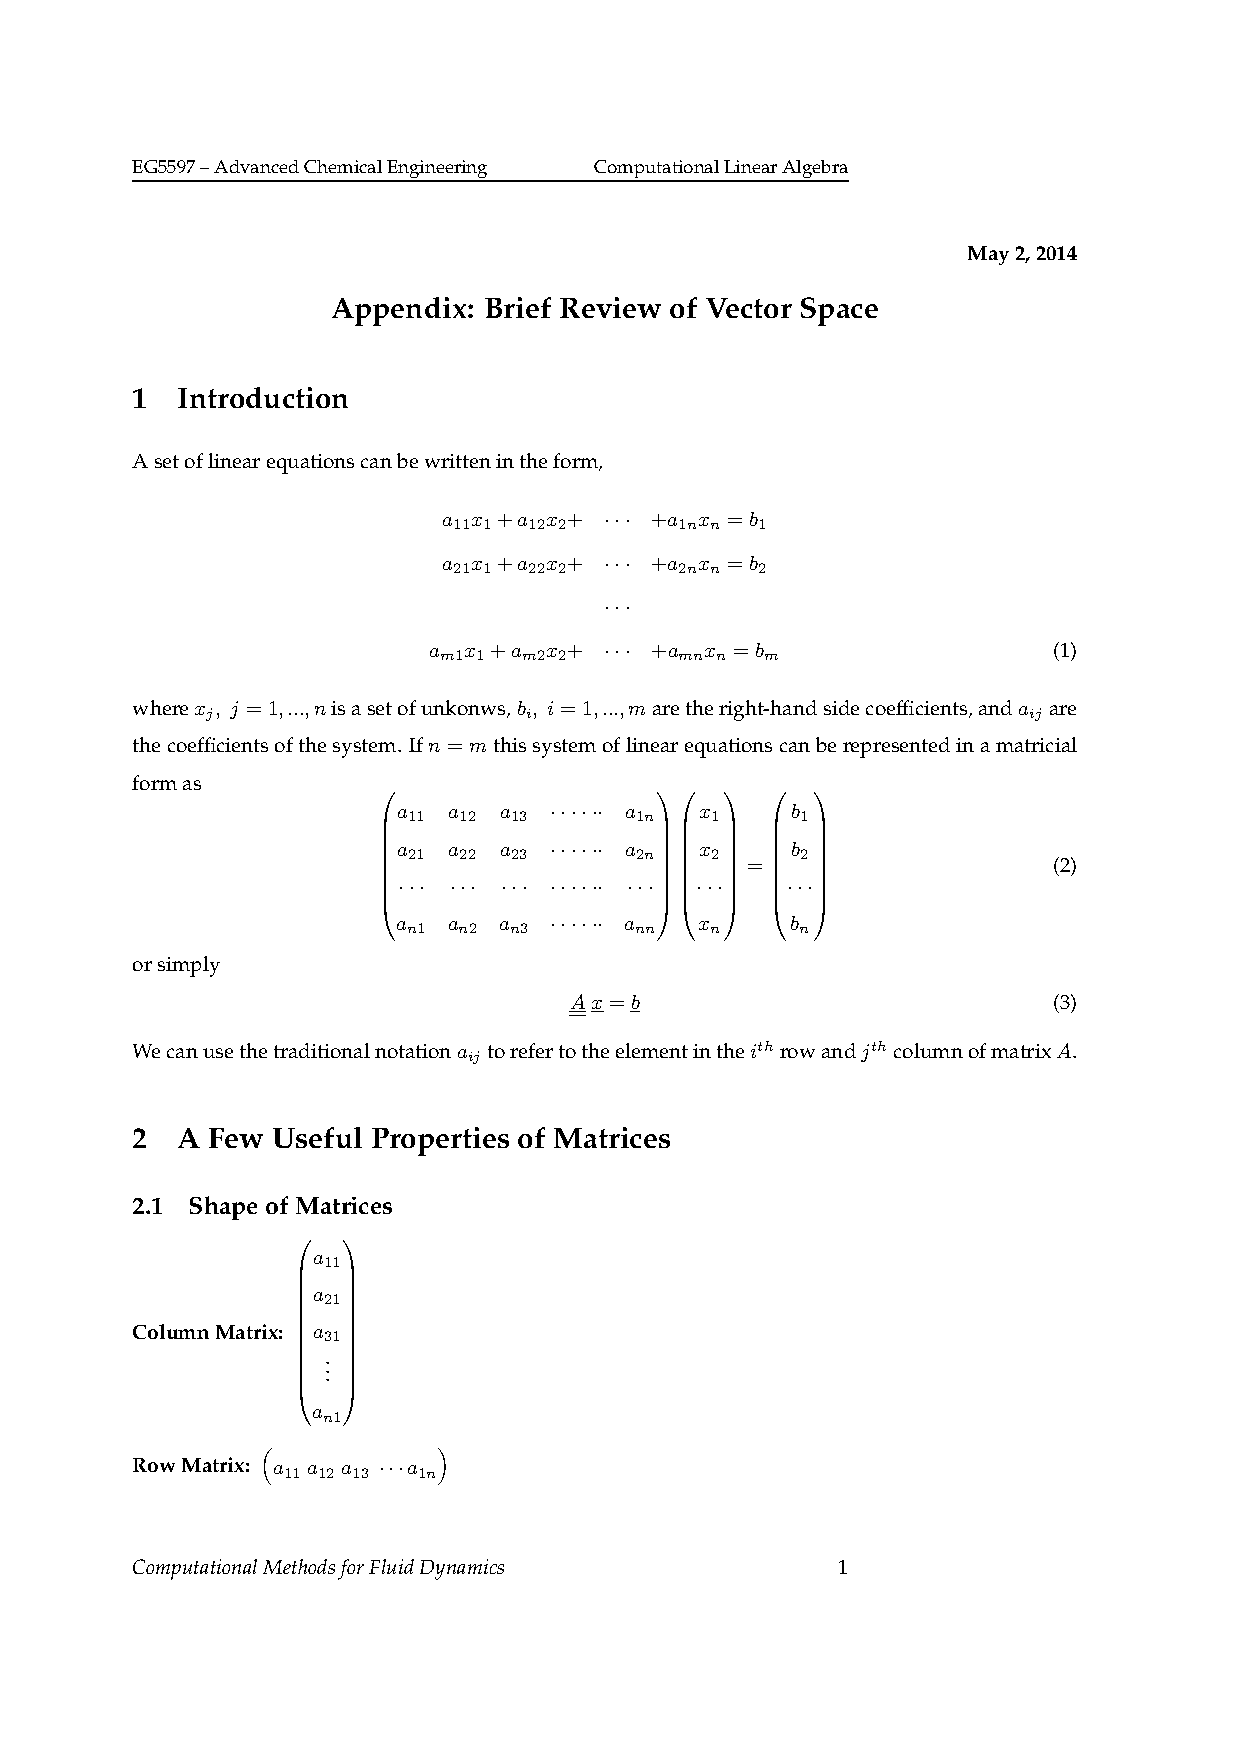
\includepdf[pages=-,fitpaper]{./ExtraNotes.pdf}
%}




\end{document}
